%\documentclass{beamer}
\documentclass[handout]{beamer}
\usetheme{Marburg}
\useoutertheme{infolines}
\newcommand{\answers}{1}

\usepackage{amsmath}
\usepackage{caption}
\usepackage{color}
\usepackage{enumerate}
\usepackage{listings}
\usepackage{hyperref}
\usepackage{mathrsfs}
\usepackage{natbib}
\usepackage{url}

\providecommand{\all}{\ \forall \ }
\providecommand{\bs}{\backslash}
\providecommand{\e}{\varepsilon}
\providecommand{\E}{\ \exists \ }
\providecommand{\lm}[2]{\lim_{#1 \rightarrow #2}}
\providecommand{\m}[1]{\mathbb{#1}}
\providecommand{\nv}{{}^{-1}}
\providecommand{\ov}[1]{\overline{#1}}
\providecommand{\p}{\newpage}
\providecommand{\q}{$\quad$ \newline}
\providecommand{\rt}{\rightarrow}
\providecommand{\Rt}{\Rightarrow}
\providecommand{\vc}[1]{\boldsymbol{#1}}
\providecommand{\wh}[1]{\widehat{#1}}

\hypersetup{colorlinks,linkcolor=,urlcolor=blue}
\numberwithin{equation}{section}

\definecolor{dkgreen}{rgb}{0,0.6,0}
\definecolor{gray}{rgb}{0.5,0.5,0.5}
\definecolor{mauve}{rgb}{0.58,0,0.82}

\lstset{ 
  language=C,                % the language of the code
  basicstyle= \tiny,           % the size of the fonts that are used for the code
  numbers=left,
  numberfirstline=true,
  numbersep=5pt,                  % how far the line-numbers are from the code
  backgroundcolor=\color{white},      % choose the background color. You must add \usepackage{color}
  showspaces=false,               % show spaces adding particular underscores
  showstringspaces=false,         % underline spaces within strings
  showtabs=false,                 % show tabs within strings adding particular underscores
  frame=lrb,                   % adds a frame around the code
  rulecolor=\color{black},        % if not set, the frame-color may be changed on line-breaks within not-black text 
  tabsize=2,                      % sets default tabsize to 2 spaces
  captionpos=t,                   % sets the caption-position 
  breaklines=true,                % sets automatic line breaking
  breakatwhitespace=false,        % sets if automatic breaks should only happen at whitespace
  %title=\lstname,                   % show the filename of files included with \lstinputlisting;
  keywordstyle=\color{blue},          % keyword style
  commentstyle=\color{gray},       % comment style
  stringstyle=\color{dkgreen},         % string literal style
  escapeinside={\%*}{*)},            % if you want to add LaTeX within your code
  morekeywords={*, ...},               % if you want to add more keywords to the set
  xleftmargin=0.2in, % left horizontal offset of caption box
  xrightmargin=-.03in % right horizontal offset of caption box
}

%\DeclareCaptionFont{white}{\color{white}}
%\DeclareCaptionFormat{listing}{\parbox{\textwidth}{\colorbox{gray}{\parbox{\textwidth}{#1#2#3}}\vskip-0.05in}}
%\captionsetup[lstlisting]{format = listing, labelfont = white, textfont = white}
%For caption-free listings, comment out the 3 lines above and uncomment the 2 lines below.
 \captionsetup{labelformat = empty, labelsep = none}
 \lstset{frame = single}

\title{CUDA C: K-means and MCMC}
\author{Will Landau}
\date{October 7, 2013}
\institute{Iowa State University}

\begin{document}

\begin{frame}
\titlepage
 \end{frame}

\begin{frame}
\frametitle{Outline}
\tableofcontents
\end{frame}
 
 \AtBeginSection[]
{
   \begin{frame}
       \frametitle{Outline}
       \tableofcontents[currentsection]
   \end{frame}
}

\section{Lloyd's K-means algorithm}

\begin{frame}
\frametitle{Lloyd's K-means algorithm}
\begin{itemize}
\item Cluster $N$ vectors in Euclidian space into $K$ groups. 
\end{itemize}

\begin{center}
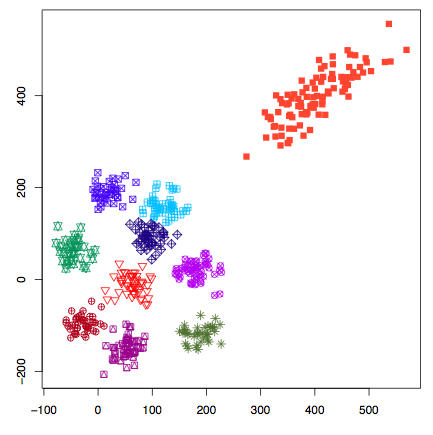
\includegraphics[scale=.4]{../../fig/kmeans0.png}
\end{center}
\end{frame}

\begin{frame}
\frametitle{Step 1: choose initial cluster centers.}
\begin{center}
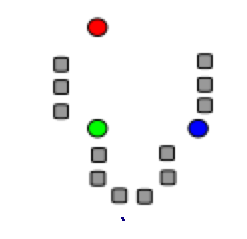
\includegraphics[scale=.6]{../../fig/kmeans1.png}
\end{center}
\begin{itemize}
\item The circles are the cluster means, the squares are the data points, and the color indicates the cluster.
\end{itemize}
\end{frame}

\begin{frame}
\frametitle{Step 2: assign each data point (square) to its closest center (circle).}
\begin{center}
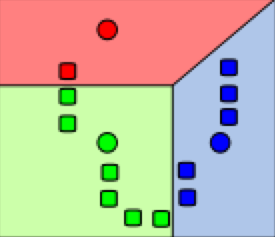
\includegraphics[scale=.6]{../../fig/kmeans2.png}
\end{center}
\end{frame}

\begin{frame}
\frametitle{Step 3: update the cluster centers to be the within-cluster data means.}
\begin{center}
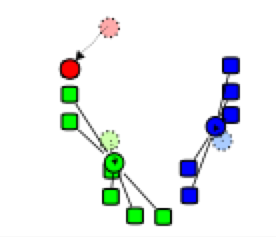
\includegraphics[scale=.6]{../../fig/kmeans3.png}
\end{center}
\end{frame}

\begin{frame}
\frametitle{Repeat step 2: reassign points to their closest cluster centers.}
\begin{center}
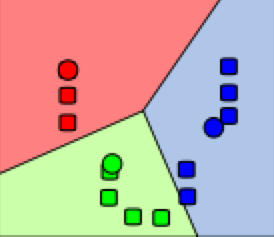
\includegraphics[scale=.6]{../../fig/kmeans4.png}
\end{center}
\begin{itemize}
\item $\ldots$ and repeat until convergence.
\end{itemize}
\end{frame}

\begin{frame}
\frametitle{Parallel K-means}
\begin{itemize}
\item Step 2: assign points to closest cluster centers
\begin{itemize}
\pause \item Spawn $N$ blocks with $K$ threads each.
\pause \item Let thread $(n, k)$ compute the distance between data point $n$ and cluster center $k$.
\pause \item Synchronize threads within each block.
\pause \item Let thread $(n, 1)$ assign data point $n$ to its nearest cluster center.
\end{itemize}
\pause \item Step 3: recompute cluster centers
\begin{itemize}
\pause \item Spawn one block for each cluster.
\pause \item Within each block, compute the mean of the data in the corresponding cluster.
\end{itemize}
\end{itemize}
\end{frame}


\begin{frame}[fragile]
\frametitle{{\tt gpu\_kmeans.cu}}
\begin{lstlisting}[name=km]
#include <stdio.h>
#include <stdlib.h>

#define I(row, col, ncols) (row * ncols + col)

#define CUDA_CALL(x) {if((x) != cudaSuccess){ \
  printf("CUDA error at %s:%d\n",__FILE__,__LINE__); \
  printf("  %s\n", cudaGetErrorString(cudaGetLastError())); \
  exit(EXIT_FAILURE);}} 
\end{lstlisting}
\end{frame}

\begin{frame}[fragile]
\frametitle{{\tt gpu\_kmeans.cu}: step 2}
\begin{lstlisting}[name=km]
__global__ void get_dst(float *dst, float *x, float *y, 
			float *mu_x, float *mu_y){
  int i = blockIdx.x;
  int j = threadIdx.x;

  dst[I(i, j, blockDim.x)] = (x[i] - mu_x[j]) * (x[i] - mu_x[j]);
  dst[I(i, j, blockDim.x)] += (y[i] - mu_y[j]) * (y[i] - mu_y[j]); 
}

__global__ void regroup(int *group, float *dst, int k){
  int i = blockIdx.x;
  int j;
  float min_dst;
  
  min_dst = dst[I(i, 0, k)];
  group[i] = 1;

  for(j = 1; j < k; ++j){
    if(dst[I(i, j, k)] < min_dst){
      min_dst = dst[I(i, j, k)];
      group[i] = j + 1;
    }
  }
}
\end{lstlisting}
\end{frame}





\begin{frame}[fragile]
\frametitle{{\tt gpu\_kmeans.cu}: step 3}
\begin{lstlisting}[name=km]
__global__ void clear(float *sum_x, float *sum_y, int *nx, int *ny){
  int j = threadIdx.x;
  
  sum_x[j] = 0;
  sum_y[j] = 0;
  nx[j] = 0;
  ny[j] = 0;
}

__global__ void recenter_step1(float *sum_x, float *sum_y, int *nx, int *ny,
			       float *x, float *y, int *group, int n){
  int i;
  int j = threadIdx.x;

  for(i = 0; i < n; ++i){
    if(group[i] == (j + 1)){
      sum_x[j] += x[i];
      sum_y[j] += y[i];
      nx[j]++;
      ny[j]++;
    }
  }               
}
\end{lstlisting}
\end{frame}


\begin{frame}[fragile]
\frametitle{{\tt gpu\_kmeans.cu}: step 3}
\begin{lstlisting}[name=km]
__global__ void recenter_step2(float *mu_x, float *mu_y, float *sum_x,
			       float *sum_y, int *nx, int *ny){
  int j = threadIdx.x;

  mu_x[j] = sum_x[j]/nx[j];
  mu_y[j] = sum_y[j]/ny[j];
}

void kmeans(int nreps, int n, int k,
            float *x_d, float *y_d, float *mu_x_d, float *mu_y_d,
            int *group_d, int *nx_d, int *ny_d,
            float *sum_x_d, float *sum_y_d, float *dst_d){
  int i;
  for(i = 0; i < nreps; ++i){
    get_dst<<<n,k>>>(dst_d, x_d, y_d, mu_x_d, mu_y_d);
    regroup<<<n,1>>>(group_d, dst_d, k);
    clear<<<1,k>>>(sum_x_d, sum_y_d, nx_d, ny_d);
    recenter_step1<<<1,k>>>(sum_x_d, sum_y_d, nx_d, ny_d, x_d, y_d, group_d, n);
    recenter_step2<<<1,k>>>(mu_x_d, mu_y_d, sum_x_d, sum_y_d, nx_d, ny_d);
  }
}

void read_data(float **x, float **y, float **mu_x, float **mu_y, int *n, int *k);
void print_results(int *group, float *mu_x, float *mu_y, int n, int k);
\end{lstlisting}
\end{frame}


\begin{frame}[fragile]
\frametitle{{\tt gpu\_kmeans.cu}}
\begin{lstlisting}[name=km]
int main(){
  /* cpu variables */
  int n; /* number of points */
  int k; /* number of clusters */
  int *group;
  float *x = NULL, *y = NULL, *mu_x = NULL, *mu_y = NULL;

  /* gpu variables */
  int *group_d, *nx_d, *ny_d;
  float *x_d, *y_d, *mu_x_d, *mu_y_d, *sum_x_d, *sum_y_d, *dst_d;

  /* read data from files on cpu */
  read_data(&x, &y, &mu_x, &mu_y, &n, &k);

  /* allocate cpu memory */
  group = (int*) malloc(n*sizeof(int));
  
  /* allocate gpu memory */
  CUDA_CALL(cudaMalloc((void**) &group_d,n*sizeof(int)));
  CUDA_CALL(cudaMalloc((void**) &nx_d, k*sizeof(int)));
  CUDA_CALL(cudaMalloc((void**) &ny_d, k*sizeof(int)));
  CUDA_CALL(cudaMalloc((void**) &x_d, n*sizeof(float)));
  CUDA_CALL(cudaMalloc((void**) &y_d, n*sizeof(float)));
  CUDA_CALL(cudaMalloc((void**) &mu_x_d, k*sizeof(float)));
  CUDA_CALL(cudaMalloc((void**) &mu_y_d, k*sizeof(float)));
  CUDA_CALL(cudaMalloc((void**) &sum_x_d, k*sizeof(float)));
  CUDA_CALL(cudaMalloc((void**) &sum_y_d, k*sizeof(float)));
  CUDA_CALL(cudaMalloc((void**) &dst_d, n*k*sizeof(float)));
\end{lstlisting}
\end{frame}

\begin{frame}[fragile]
\frametitle{{\tt gpu\_kmeans.cu}}
\begin{lstlisting}[name=km]
  /* write data to gpu */
  CUDA_CALL(cudaMemcpy(x_d, x, n*sizeof(float), cudaMemcpyHostToDevice));
  CUDA_CALL(cudaMemcpy(y_d, y, n*sizeof(float), cudaMemcpyHostToDevice));
  CUDA_CALL(cudaMemcpy(mu_x_d, mu_x, k*sizeof(float), cudaMemcpyHostToDevice));
  CUDA_CALL(cudaMemcpy(mu_y_d, mu_y, k*sizeof(float), cudaMemcpyHostToDevice));

  /* perform kmeans */
  kmeans(10, n, k, x_d, y_d, mu_x_d, mu_y_d, group_d, nx_d, ny_d, sum_x_d, sum_y_d, dst_d);
  
  /* read back data from gpu */
  CUDA_CALL(cudaMemcpy(group, group_d, n*sizeof(int), cudaMemcpyDeviceToHost));
  CUDA_CALL(cudaMemcpy(mu_x, mu_x_d, k*sizeof(float), cudaMemcpyDeviceToHost));
  CUDA_CALL(cudaMemcpy(mu_y, mu_y_d, k*sizeof(float), cudaMemcpyDeviceToHost));

  /* print results and clean up */  
  print_results(group, mu_x, mu_y, n, k);
\end{lstlisting}
\end{frame}

\begin{frame}[fragile]
\frametitle{{\tt gpu\_kmeans.cu}}
\begin{lstlisting}[name=km]
  free(x);
  free(y);
  free(mu_x);
  free(mu_y);
  free(group);

  CUDA_CALL(cudaFree(x_d));
  CUDA_CALL(cudaFree(y_d));
  CUDA_CALL(cudaFree(mu_x_d));
  CUDA_CALL(cudaFree(mu_y_d));
  CUDA_CALL(cudaFree(group_d));
  CUDA_CALL(cudaFree(nx_d));
  CUDA_CALL(cudaFree(ny_d));
  CUDA_CALL(cudaFree(sum_x_d));
  CUDA_CALL(cudaFree(sum_y_d));
  CUDA_CALL(cudaFree(dst_d));

  return 0;
}

\end{lstlisting}
\end{frame}

\lstset{language = bash}

\begin{frame}[fragile]
\frametitle{Compile, test, and run.}
\begin{itemize}
\item Compile CPU and GPU versions.
\begin{lstlisting}
> make
gcc kmeans.c -o kmeans -Wall -ansi -pedantic
nvcc gpu_kmeans.cu -o gpu_kmeans --compiler-options -ansi --compiler-options -Wall
\end{lstlisting}
\pause \item Always run through CUDA MEMCHECK.
\begin{lstlisting}
> cuda-memcheck ./gpu_kmeans
========= CUDA-MEMCHECK
========= ERROR SUMMARY: 0 errors
\end{lstlisting}
\pause \item Check CPU side with Valgrind. Ignore ``errors" and apparent memory leaks on the GPU side.
\begin{lstlisting}
> valgrind ./gpu_kmeans
==13523== Memcheck, a memory error detector
==13523== Copyright (C) 2002-2010, and GNU GPL'd, by Julian Seward et al.
==13523== Using Valgrind-3.6.0 and LibVEX; rerun with -h for copyright info
==13523== Command: ./gpu_kmeans
==13523== 
==13523== Warning: set address range perms: large range [0x800000000, 0x2100000000) (noaccess)
==13523== Warning: set address range perms: large range [0x2100000000, 0x2800000000) (noaccess)
\end{lstlisting}
\end{itemize}
\end{frame}

\begin{frame}[fragile]
\frametitle{Compile, test, and run.}
\begin{itemize}
\begin{lstlisting}
==13523== 
==13523== HEAP SUMMARY:
==13523==     in use at exit: 1,308,694 bytes in 2,469 blocks
==13523==   total heap usage: 4,479 allocs, 2,010 frees, 2,952,191 bytes allocated
==13523== 
==13523== LEAK SUMMARY:
==13523==    definitely lost: 16 bytes in 1 blocks
==13523==    indirectly lost: 0 bytes in 0 blocks
==13523==      possibly lost: 33,064 bytes in 242 blocks
==13523==    still reachable: 1,275,614 bytes in 2,226 blocks
==13523==         suppressed: 0 bytes in 0 blocks
==13523== Rerun with --leak-check=full to see details of leaked memory
==13523== 
==13523== For counts of detected and suppressed errors, rerun with: -v
==13523== ERROR SUMMARY: 0 errors from 0 contexts (suppressed: 11 from 9)
\end{lstlisting}
\pause \item Run for real.
\begin{lstlisting}
> ./gpu_kmeans
\end{lstlisting}
\end{itemize}
\end{frame}

\lstset{language = C}


\begin{frame}[fragile]
\frametitle{Initial clustering: 300 points, 3 clusters}
\begin{center}
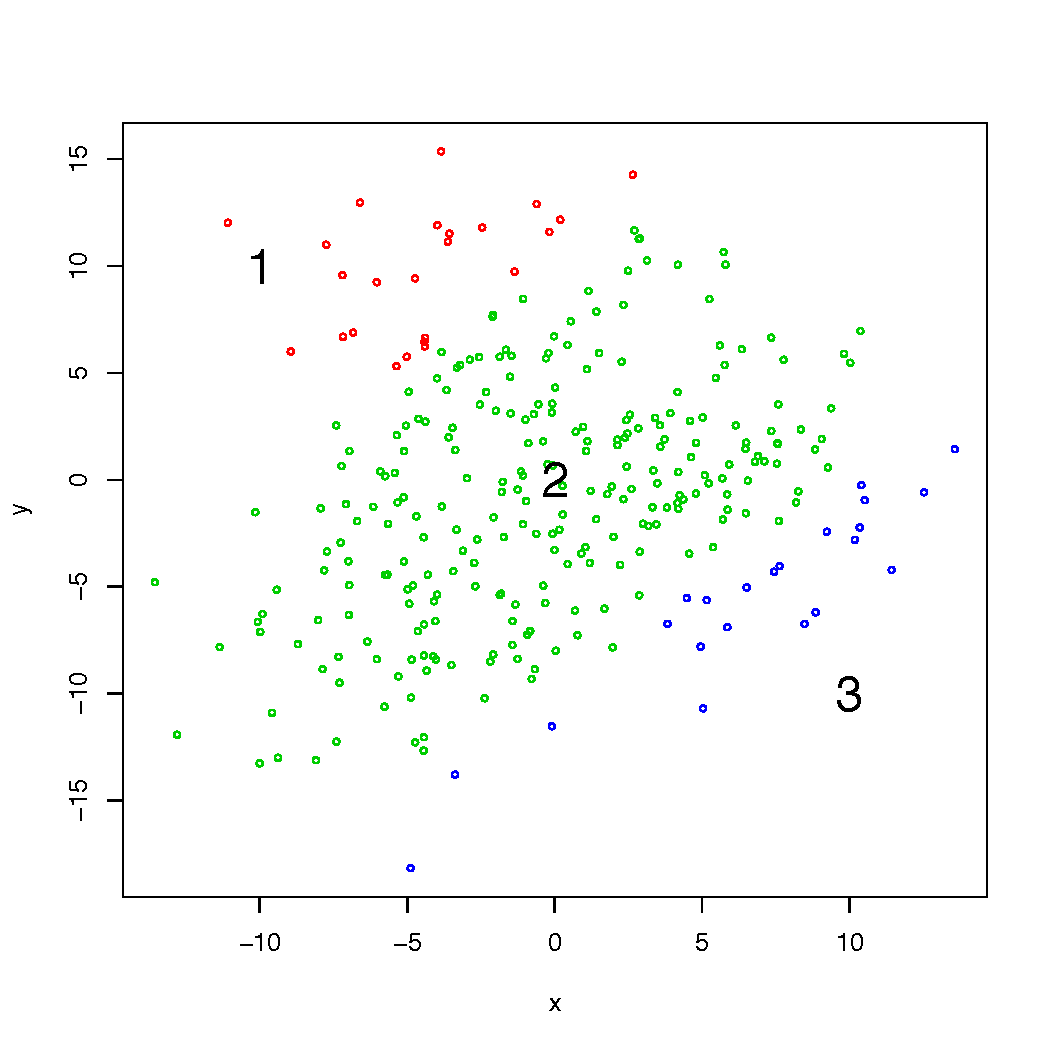
\includegraphics[scale=.5]{../../fig/kmeans-before}
\end{center}
\end{frame}

\begin{frame}[fragile]
\frametitle{Final clustering after 10 iterations}
\begin{center}
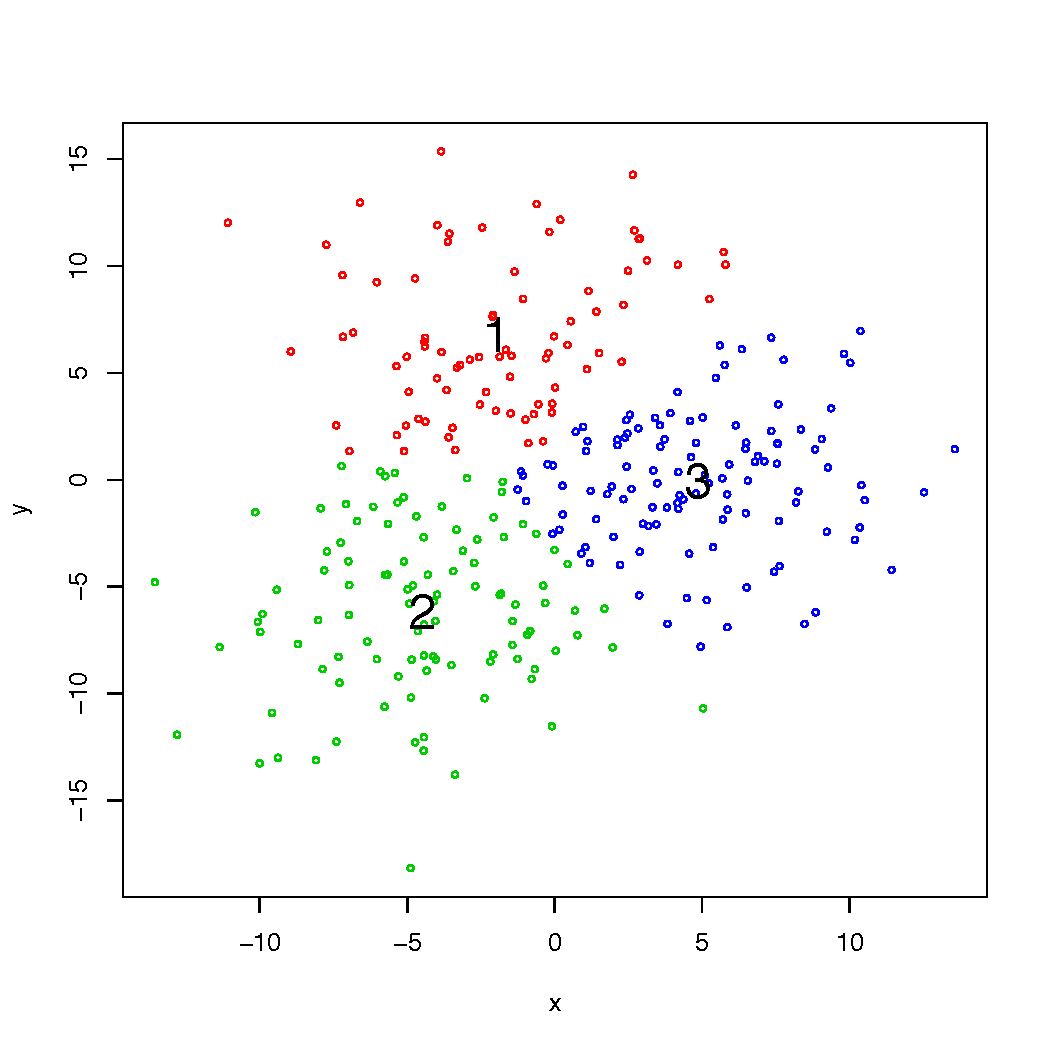
\includegraphics[scale=.5]{../../fig/kmeans-after}
\end{center}
\end{frame}

\section{Markov chain Monte Carlo}


\begin{frame}
\frametitle{Markov chain Monte Carlo}
\begin{itemize}
\item Consider a bladder cancer data set:
\begin{itemize}  \scriptsize
\pause \item Available from http://ratecalc.cancer.gov/.
\pause \item Rates of death from bladder cancer of white males from 2000 to 2004 in each county in the USA.
\end{itemize}
\pause \item Let:
\begin{itemize}  \scriptsize
\item $y_k$ = number of observed deaths in county $k$.
\pause \item $n_k$ = the number of person-years in county $k$ divided by 100,000.
\pause \item $\theta_k$ = expected number of deaths per 100,000 person-years.
\end{itemize} 
\pause \item The model:
\begin{align*}
\uncover<7->{y_k} &\uncover<7->{\stackrel{\text{ind}}{\sim} \text{Poisson}(n_k \cdot \theta_k)}\\
\uncover<8->{\theta_k} &\uncover<8->{\stackrel{\text{iid}}{\sim} \text{Gamma}(\alpha, \ \beta)}\\
\uncover<9->{\alpha} & \uncover<9->{\sim \text{Uniform}(0, a_0)} \\
\uncover<10->{\beta} & \uncover<10->{\sim \text{Uniform}(0, b_0)}
\end{align*}
\uncover<11->{\begin{itemize}
\item Also assume that shape $\alpha$ and rate $\beta$ are independent and fix $a_0$ and $b_0$.
\end{itemize}}
\end{itemize}
\end{frame}










\begin{frame}
\frametitle{Full conditional distributions} \scriptsize
\begin{itemize}
\item We want to sample from the joint posterior,
\end{itemize}
\begin{align*}
p(\vc{\theta}, \alpha, \beta \mid \vc{y}) &\propto p(\vc{y} \mid \vc{\theta}, \alpha, \beta) p(\vc{\theta}, \alpha, \beta) \\
&\uncover<2->{\propto p(\vc{y} \mid \vc{\theta}, \alpha, \beta) p(\vc{\theta} \mid \alpha, \beta) p(\alpha, \beta)} \\
&\uncover<3->{\propto p(\vc{y} \mid \vc{\theta}, \alpha, \beta) p(\vc{\theta} \mid \alpha, \beta) p(\alpha)p(\beta)} \\
&\uncover<4->{\propto \prod_{k = 1}^K [p(y_k \mid \theta_k, n_k) p(\theta_k \mid \alpha, \beta)] p(\alpha) p(\beta)} \\
&\uncover<5->{\propto \prod_{k = 1}^K \left [e^{-n_k \theta_k} \theta_k^{y_k} \frac{\beta^\alpha}{\Gamma(\alpha)} \theta_k^{\alpha - 1} e^{-\theta_k \beta}\right ] I(0 < \alpha < a_0) I(0 < \beta < b_0) }
\end{align*}
\begin{itemize}
\uncover<6->{\item We iteratively sample from the full conditional distributions.}
\end{itemize}
\begin{align*}
\uncover<7->{\alpha} &\uncover<7->{\leftarrow p(\alpha \mid \vc{y}, \vc{\theta}, \beta)}  \\
\uncover<8->{\beta} &\uncover<8->{\leftarrow p(\beta \mid \vc{y}, \vc{\theta}, \alpha)} \\
\uncover<9->{\theta_k} &\uncover<9->{\leftarrow p(\theta_k \mid \vc{y}, \vc{\theta}_{-k}, \alpha, \beta) \qquad \Leftarrow \text{IN PARALLEL!}} 
\end{align*}
\end{frame}

\begin{frame}
\frametitle{Full conditional distributions} 
\begin{align*}
\uncover<2->{p(\theta_k \mid \vc{y}, \vc{\theta_{-k}}, \alpha, \beta)} & \uncover<2->{\propto p(\vc{\theta}, \alpha, \beta \mid \vc{y})} \\
&\uncover<3->{\propto e^{-n_k \theta_k} \theta_k^{y_k} \theta_k^{\alpha - 1} e^{- \theta_k} \beta} \\
&\uncover<4->{= \theta_k^{y_k + \alpha - 1} e^{-\theta_k(n_k + \beta)}} \\
&\uncover<5->{\propto \text{Gamma}(y_k + \alpha, \ n_k + \beta)}
\end{align*}
\end{frame}


\begin{frame} 
\frametitle{Conditional distributions of $\alpha$ and $\beta$} \small
\begin{align*}
p(\alpha \mid \vc{y}, \vc{\theta}, \beta) &\propto p(\vc{\theta}, \alpha, \beta \mid \vc{y}) \\
&\uncover<2->{\propto \prod_{k = 1}^K \left [ \theta_k^{\alpha - 1} \frac{\beta^\alpha}{\Gamma(\alpha)} \right ] I(0 < \alpha < a_0)} \\
&\uncover<3->{=\left (\prod_{k = 1}^K \theta_k \right )^\alpha \beta^{K \alpha} \Gamma(\alpha)^{-K} I(0 < \alpha < a_0)} \\ \\
\uncover<4->{p(\beta \mid \vc{y}, \vc{\theta}, \alpha)} &\uncover<4->{\propto p(\vc{\theta}, \alpha, \beta \mid \vc{y})} \\
&\uncover<5->{\propto \prod_{k = 1}^K \left [ e^{-\theta_k \beta} \beta^\alpha \right ] I(0 < \beta < b_0)} \\
&\uncover<6->{=\beta^{K \alpha} e^{- \beta \sum_{k = 1}^K \theta_k} I(0 < \beta < b_0)} \\
&\uncover<7->{\propto \text{Gamma}\left (K \alpha + 1, \ \sum_{k = 1}^K \theta_k \right) I(0 < \beta < b_0)}
\end{align*}
\end{frame}


\begin{frame}
\frametitle{Summarizing the Gibbs sampler}
\begin{enumerate}
\item Sample $\vc{\theta}$ from from its full conditional.
\begin{itemize}
\pause \item Draw the $\theta_k$'s \emph{in parallel} from independent Gamma($y_k + \alpha$, $n_k + \beta$) distributions.
\pause \item In other words, assign each thread to draw an individual $\theta_k$ from its Gamma($y_k + \alpha$, $n_k + \beta$) distribution.
\end{itemize}
\pause \item Sample $\alpha$ from its full conditional using a random walk Metropolis step.
\pause \item Sample $\beta$ from its full conditional (truncated Gamma) using the inverse cdf method if $b_0$ is low or a non-truncated Gamma if $b_0$ is high.
\end{enumerate}

\end{frame}









\begin{frame}
\frametitle{The gamma sampler for $\beta$ and $\theta_1, \ldots, \theta_K$}
\begin{itemize} \small
\item Taken from Marsaglia and Tsang (2001).
\pause \item Rejection sampler with acceptance rate $\ge 95\%$ when the shape parameter is $\ge 1$.
\pause \item Steps for a Gamma($a$, 1) sampler:
\begin{enumerate} \small
\pause \item Let $d = a - 1/3$ and $c = 1 / \sqrt{9 d}$.
\pause \item Draw $x \sim $ Normal(0, 1) and let $v = (1 + c \cdot x)^3$. Repeat if $v \le 0$.
\pause \item Let $u \sim $ Uniform(0, 1).
\pause \item If $u < 1 - 0.0331 \cdot x^4$, return $d \cdot v$.
\pause \item If $\log(u) < 0.5 \cdot x^2 + d \cdot (1 - v + \log(v))$, return $d \cdot v$.
\pause \item Go to step 2.
\end{enumerate}
\end{itemize}
\end{frame}

\begin{frame}
\frametitle{The metropolis step for $\alpha$}
\begin{itemize} \scriptsize
\item The goal is to sample from the full conditional distribution,
\begin{align*}
p(\alpha \mid \vc{y}, \vc{\theta}, \beta) \propto \left ( \prod_{k = 1}^K \theta_k \right )^\alpha \beta^{K \alpha} \Gamma(\alpha)^{-K} I(0 < \alpha < a_0)
\end{align*}
\pause \item Let $\alpha^{(j)}$ be the last sampled value of $\alpha$. Sample $\alpha^{(j + 1)}$ as follows:

\begin{enumerate} \scriptsize
\pause \item Draw $\alpha^* \sim N(\alpha^{(j)}, \ \sigma^2$), where $\sigma^2$ is a tuning parameter.
\pause \item If $\alpha^* < 0$ or $\alpha^* > a_0$, let $p = 0$. Otherwise,
\end{enumerate}

\pause \begin{align*}
p = \frac{p(\alpha^* \mid \vc{y}, \vc{\theta}, \beta)}{p(\alpha^{(j)} \mid \vc{y}, \vc{\theta}, \beta)} = \left ( \prod_{k = 1}^K \theta_k \right )^{\alpha^* - \alpha^{(j)}} \beta^{K(\alpha^* - \alpha^{(j)})} \left( \frac{\Gamma(\alpha^*)}{\Gamma(\alpha^{(j)})} \right )^{-K}
\end{align*}
\begin{enumerate} \setcounter{enumi}{2} \scriptsize
\pause \item Draw $u \sim U(0, 1)$.
\pause \item If $u < p$, $\alpha^{(j + 1)} = \alpha^*$. Otherwise, $\alpha^{(j + 1)} = \alpha^{(j)}$.
\pause \item Raise $\sigma^2$ if $\alpha^*$ was accepted and lower $\sigma^2$ if $\alpha^*$ was rejected. The optimal acceptance rate is roughly 44\%.
\end{enumerate}
\end{itemize}
\end{frame}













\begin{frame}[fragile]
\frametitle{Zebulun Arendsee's implementation}
\begin{lstlisting}[name=mc]
/*
Created by Zebulun Arendsee.
March 26, 2013

Modified by Will Landau.
June 30, 2013
will-landau.com
landau@iastate.edu

This program implements a MCMC algorithm for the following hierarchical
model:

y_k     ~ Poisson(n_k * theta_k)     k = 1, ..., K
theta_k ~ Gamma(a, b)
a       ~ Unif(0, a0)
b       ~ Unif(0, b0) 

We let a0 and b0 be arbitrarily large.

Arguments:
    1) input filename
        With two space delimited columns holding integer values for
        y and float values for n.
    2) number of trials (1000 by default)

Output: A comma delimited file containing a column for a, b, and each
theta. All output is written to stdout. */
\end{lstlisting}
\end{frame}

\begin{frame}[fragile]
\frametitle{Zebulun Arendsee's implementation}
\begin{lstlisting}[name=mc]
/*
Example dataset:

$ head -3 data.txt
4 0.91643
23 3.23709
7 0.40103

 Example of compilation and execution:

$ nvcc gibbs_metropolis.cu -o gibbs
$ ./gibbs mydata.txt 2500 > output.csv
$

This code borrows from the nVidia developer zone documentation, 
specifically http://docs.nvidia.com/cuda/curand/index.html#topic_1_2_1
*/

#include <stdio.h>
#include <stdlib.h>
#include <cuda.h>
#include <math.h>
#include <curand_kernel.h>
#include <thrust/reduce.h>

#define PI 3.14159265359f
#define THREADS_PER_BLOCK 64
\end{lstlisting}
\end{frame}

\begin{frame}[fragile]
\frametitle{Zebulun Arendsee's implementation}
\begin{lstlisting}[name=mc]
#define CUDA_CALL(x) {if((x) != cudaSuccess){ \
  printf("CUDA error at %s:%d\n",__FILE__,__LINE__); \
  printf("  %s\n", cudaGetErrorString(cudaGetLastError())); \
  exit(EXIT_FAILURE);}} 

#define CURAND_CALL(x) {if((x) != CURAND_STATUS_SUCCESS) { \
  printf("Error at %s:%d\n",__FILE__,__LINE__); \
  printf("  %s\n", cudaGetErrorString(cudaGetLastError())); \
  exit(EXIT_FAILURE);}}

__host__ void load_data(int argc, char **argv, int *K, int **y, float **n);

__host__ float sample_a(float a, float b, int K, float sum_logs);
__host__ float sample_b(float a, int K, float flat_sum);

__host__ float rnorm();
__host__ float rgamma(float a, float b);

__device__ float rgamma(curandState *state, int id, float a, float b);

__global__ void sample_theta(curandState *state, float *theta, float *log_theta, int *y, float *n, float a, float b, int K);
__global__ void setup_kernel(curandState *state, unsigned int seed, int);
\end{lstlisting}
\end{frame}

\begin{frame}[fragile]
\frametitle{Zebulun Arendsee's implementation}
\begin{lstlisting}[name=mc]
int main(int argc, char **argv){

  curandState *devStates;
  float a, b, flat_sum, sum_logs, *n, *dev_n, *dev_theta, *dev_log_theta;
  int i, K, *y, *dev_y, nBlocks, trials = 1000;

  if(argc > 2)
    trials = atoi(argv[2]);

  load_data(argc, argv, &K, &y, &n);


  /*------ Allocate memory -----------------------------------------*/

  CUDA_CALL(cudaMalloc((void **)&dev_y, K * sizeof(int)));
  CUDA_CALL(cudaMemcpy(dev_y, y, K * sizeof(int), 
            cudaMemcpyHostToDevice));

  CUDA_CALL(cudaMalloc((void **)&dev_n, K * sizeof(float)));
  CUDA_CALL(cudaMemcpy(dev_n, n, K * sizeof(float), 
            cudaMemcpyHostToDevice));

  /* Allocate space for theta and log_theta on device and host */
  CUDA_CALL(cudaMalloc((void **)&dev_theta, K * sizeof(float)));
  CUDA_CALL(cudaMalloc((void **)&dev_log_theta, K * sizeof(float)));

  /* Allocate space for random states on device */
  CUDA_CALL(cudaMalloc((void **)&devStates, K * sizeof(curandState)));
\end{lstlisting}
\end{frame}

\begin{frame}[fragile]
\frametitle{Zebulun Arendsee's implementation}
\begin{lstlisting}[name=mc]
  /*------ Setup random number generators (one per thread) ---------*/

  nBlocks = (K + THREADS_PER_BLOCK - 1) / THREADS_PER_BLOCK;
  setup_kernel<<<nBlocks, THREADS_PER_BLOCK>>>(devStates, 0, K);

\end{lstlisting}
\end{frame}

\begin{frame}[fragile]
\frametitle{Zebulun Arendsee's implementation}
\begin{lstlisting}[name=mc]
  /*------ MCMC ----------------------------------------------------*/
    
  printf("alpha, beta\n");

  /* starting values of hyperparameters */
  a = 20; 
  b = 1; 

  /* Steps of MCMC */  
  for(i = 0; i < trials; i++){    
    sample_theta<<<nBlocks, THREADS_PER_BLOCK>>>(devStates, dev_theta, dev_log_theta, dev_y, dev_n, a, b, K);

    /* print hyperparameters. */
    printf("%f, %f\n", a, b);

    /* Make iterators for thetas and log thetas. */
    thrust::device_ptr<float> theta(dev_theta);
    thrust::device_ptr<float> log_theta(dev_log_theta);
    
    /* Compute pairwise sums of thetas and log_thetas. */
    flat_sum = thrust::reduce(theta, theta + K);
    sum_logs = thrust::reduce(log_theta, log_theta + K);
  
    /* Sample hyperparameters. */
    a = sample_a(a, b, K, sum_logs);
    b = sample_b(a, K, flat_sum);
  }
\end{lstlisting}
\end{frame}

\begin{frame}[fragile]
\frametitle{Zebulun Arendsee's implementation}
\begin{lstlisting}[name=mc]
  /*------ Free Memory -------------------------------------------*/

  free(y);
  free(n);

  CUDA_CALL(cudaFree(devStates));
  CUDA_CALL(cudaFree(dev_theta));
  CUDA_CALL(cudaFree(dev_log_theta));
  CUDA_CALL(cudaFree(dev_y));
  CUDA_CALL(cudaFree(dev_n));

  return EXIT_SUCCESS;
}
\end{lstlisting}
\end{frame}

\begin{frame}[fragile]
\frametitle{Zebulun Arendsee's implementation}
\begin{lstlisting}[name=mc]
/*
 *  Metropolis algorithm for producing random a values. 
 *  The proposal distribution in normal with a variance that
 *  is adjusted at each step.
 */
 
__host__ float sample_a(float a, float b, int K, float sum_logs){

  static float sigma = 2;
  float U, log_acceptance_ratio, proposal = rnorm() * sigma + a;

  if(proposal <= 0) 
    return a;

  log_acceptance_ratio = (proposal - a) * sum_logs +
                         K * (proposal - a) * log(b) -
                         K * (lgamma(proposal) - lgamma(a));

  U = rand() / float(RAND_MAX);

  if(log(U) < log_acceptance_ratio){
    sigma *= 1.1;
    return proposal;
  } else {
    sigma /= 1.1;
    return a;
  }
}
\end{lstlisting}
\end{frame}

\begin{frame}[fragile]
\frametitle{Zebulun Arendsee's implementation}
\begin{lstlisting}[name=mc]
/*
 *  Sample b from a gamma distribution.
 */

__host__ float sample_b(float a, int K, float flat_sum){

  float hyperA = K * a + 1;
  float hyperB = flat_sum;
  return rgamma(hyperA, hyperB);
}

 
__host__ float rnorm(){

  float U1 = rand() / float(RAND_MAX);
  float U2 = rand() / float(RAND_MAX);
  float V1 = sqrt(-2 * log(U1)) * cos(2 * PI * U2);
  /* float V2 = sqrt(-2 * log(U2)) * cos(2 * PI * U1); */
  return V1;
}
\end{lstlisting}
\end{frame}

\begin{frame}[fragile]
\frametitle{Zebulun Arendsee's implementation}
\begin{lstlisting}[name=mc]
__host__ float rgamma(float a, float b){

  float d = a - 1.0 / 3;
  float Y, U, v;

  while(1){
    Y = rnorm();
    v = pow((1 + Y / sqrt(9 * d)), 3);

    /* Necessary to avoid taking the log of a negative number later. */
    if(v <= 0) 
      continue;
        
    U = rand() / float(RAND_MAX);

    /* Accept the sample under the following condition. 
       Otherwise repeat loop. */
    if(log(U) < 0.5 * pow(Y,2) + d * (1 - v + log(v)))
            return d * v / b;
  }
}
\end{lstlisting}
\end{frame}

\begin{frame}[fragile]
\frametitle{Zebulun Arendsee's implementation}
\begin{lstlisting}[name=mc]
__device__ float rgamma(curandState *state, int id, float a, float b){

  float d = a - 1.0 / 3;
  float Y, U, v;

  while(1){   
    Y = curand_normal(&state[id]);
    v = pow((1 + Y / sqrt(9 * d)), 3);

    /* Necessary to avoid taking the log of a negative number later. */
    if(v <= 0) 
      continue;
        
    U = curand_uniform(&state[id]);

    /* Accept the sample under the following condition. 
       Otherwise repeat loop. */
    if(log(U) < 0.5 * pow(Y,2) + d * (1 - v + log(v)))
      return d * v / b;
  }
}
\end{lstlisting}
\end{frame}



\begin{frame}[fragile]
\frametitle{Zebulun Arendsee's implementation}
\begin{lstlisting}[name=mc]
/*
 *  Sample each theta from the appropriate gamma distribution
 */
 
__global__ void sample_theta(curandState *state,  float *theta, 
                             float *log_theta, int *y, float *n, float a, float b, int K){
                             
  int id = threadIdx.x + blockIdx.x * blockDim.x;
  float hyperA, hyperB;
    
  if(id < K){
    hyperA = a + y[id];
    hyperB = b + n[id];
    theta[id] = rgamma(state, id, hyperA, hyperB);
    log_theta[id] = log(theta[id]);
  }
}

/* 
 *  Initialize GPU random number generators 
 */
 
__global__ void setup_kernel(curandState *state, unsigned int seed, int K){
  int id = threadIdx.x + blockIdx.x * blockDim.x;
  if(id < K)
    curand_init(seed, id, 0, &state[id]);
}
\end{lstlisting}
\end{frame}

\lstset{language = bash, basicstyle = \tiny}

\begin{frame}[fragile]
\frametitle{Compile, test, and run.}
\begin{itemize}
\item Compile, requiring compute capability 2.0 or above. 
\begin{lstlisting}
> nvcc -arch=sm_20 gibbs_metropolis.cu -o gibbs_metropolis
\end{lstlisting}
\pause \item Always check with CUDA MEMCHECK.
\begin{lstlisting}
> cuda-memcheck ./gibbs_metropolis smallData.txt 10
========= CUDA-MEMCHECK
alpha, beta
19.070215, 1.226651
19.441961, 1.521381
16.017313, 1.413954
11.898635, 1.253917
11.898635, 1.767045
13.532320, 1.783169
13.532320, 1.648099
13.532320, 2.005379
13.532320, 2.136331
12.914721, 1.408586
========= ERROR SUMMARY: 0 errors 
\end{lstlisting}
\end{itemize}
\end{frame}

\begin{frame}[fragile]
\frametitle{Compile, test, and run.}
\begin{itemize}
\item Check CPU side with Valgrind. Ignore ``errors" from GPU code.
\begin{lstlisting}
> valgrind ./gibbs_metropolis smallData.txt 10
==12942== Memcheck, a memory error detector
==12942== Copyright (C) 2002-2010, and GNU GPL'd, by Julian Seward et al.
==12942== Using Valgrind-3.6.0 and LibVEX; rerun with -h for copyright info
==12942== Command: ./gibbs_metropolis smallData.txt 10
==12942== 
==12942== Warning: set address range perms: large range [0x800000000, 0x2100000000) (noaccess)
==12942== Warning: set address range perms: large range [0x2100000000, 0x2800000000) (noaccess)
alpha, beta
19.070215, 1.226651
19.441961, 1.521381
16.017313, 1.413954
11.898635, 1.253917
11.898635, 1.767045
13.532320, 1.783169
13.532320, 1.648099
13.532320, 2.005379
13.532320, 2.136331
12.914721, 1.408586
\end{lstlisting}
\end{itemize}
\end{frame}

\begin{frame}[fragile]
\frametitle{Compile, test, and run.}
\begin{itemize}
\begin{lstlisting}
==12942== 
==12942== HEAP SUMMARY:
==12942==     in use at exit: 1,453,685 bytes in 2,647 blocks
==12942==   total heap usage: 4,175 allocs, 1,528 frees, 2,706,460 bytes allocated
==12942== 
==12942== LEAK SUMMARY:
==12942==    definitely lost: 16 bytes in 1 blocks
==12942==    indirectly lost: 0 bytes in 0 blocks
==12942==      possibly lost: 39,184 bytes in 287 blocks
==12942==    still reachable: 1,414,485 bytes in 2,359 blocks
==12942==         suppressed: 0 bytes in 0 blocks
==12942== Rerun with --leak-check=full to see details of leaked memory
==12942== 
==12942== For counts of detected and suppressed errors, rerun with: -v
==12942== ERROR SUMMARY: 0 errors from 0 contexts (suppressed: 11 from 9)
\end{lstlisting}
\pause \item Run 2 chains for real.
\begin{lstlisting}
> ./gibbs_metropolis data.txt 10000 > chain1.txt
> ./gibbs_metropolis data.txt 10000 > chain2.txt
\end{lstlisting}
\end{itemize}
\end{frame}



\begin{frame}
\frametitle{Diagnostics: Gelman-Rubin potential scale reduction factor}
\begin{align*}
\wh{R}  = \sqrt{\frac{\frac{n-1}{n} W + \frac{1}{n} B}{W}} \approx \sqrt{1 + \frac{B}{nW}}
\end{align*}
\begin{itemize}
\pause \item $n$ is the number of chains, $B$ is the between-chain variability, and $W$ is the within-chain variability.
\pause \item $\wh{R} > 1.1$ is evidence of a lack of convergence.
\pause \item For 2 chains, each with 10000 iterations (including 2000 iterations of burn-in), 
\begin{center}
\begin{tabular}{l|l|l}
& Point est $\wh{R}$ & Upper 95\% CI $\wh{R}$ \\ \hline
$\alpha$ & 1.02 & 1.08 \\
$\beta$ & 1.02 & 1.08
\end{tabular}
\end{center}
\end{itemize}
\end{frame}

\begin{frame}
\frametitle{Diagnostics: trace plots after burn-in}
\begin{center}
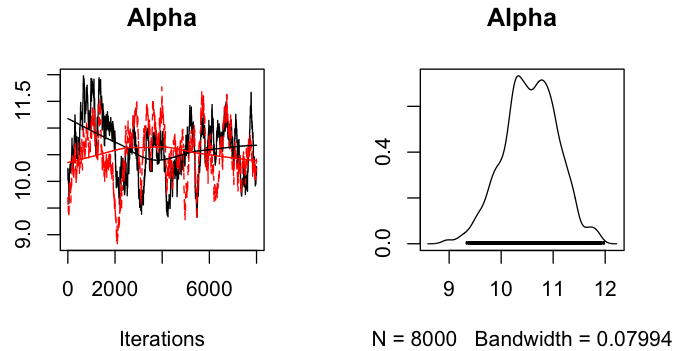
\includegraphics[scale=.3]{../../fig/mcmc-trace-alpha.png} \\
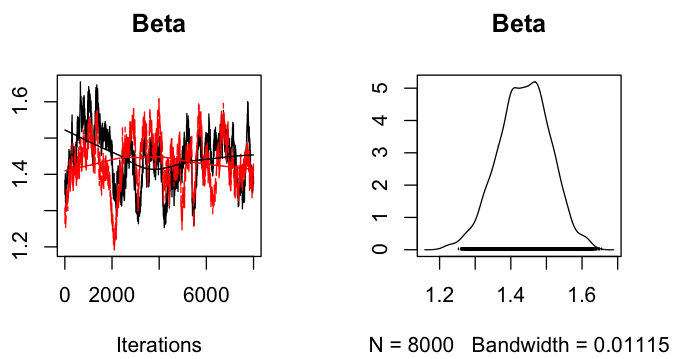
\includegraphics[scale=.3]{../../fig/mcmc-trace-beta.png}
\end{center}
\end{frame}


\begin{frame}
\frametitle{Outline}
\tableofcontents
\end{frame}

\begin{frame}
\frametitle{Resources} \small

\begin{itemize}
\item Sources:
\begin{enumerate}
\item Dr. Ranjan Maitra's STAT 580 notes.
\pause \item \href{http://jarad.me/stat544/archive.html}{Dr. Jarad Niemi's STAT 544 notes.}
\pause \item Andrew Gelman, John B. Carlin, Hal S. Stern, and Donald B. Rubin. \emph{Bayesian Data Analysis}. 2nd ed. Chapman \& Hall/CRC, 2004.
\pause \item George Marsaglia and Wai Wan Tsang. ``A Simple Method for Generating Gamma Variables." \emph{ACM Transactions on Mathematical Software} 26(3), Sept 2000. 363-372.
\end{enumerate}
\pause \item Code from today:
\begin{itemize}
\item \href{http://will-landau.com/gpu/Code/CUDA_C/kmeans/kmeans.zip}{kmeans.zip}
\item \href{http://will-landau.com/gpu/Code/CUDA_C/mcmc/mcmc.zip}{mcmc.zip}
\end{itemize}
\end{itemize}
\end{frame}



\begin{frame}
\frametitle{That's all for today.}
\begin{itemize}
\item Series materials are available at \url{http://will-landau.com/gpu}.
\end{itemize}
\end{frame}


\end{document}